% Options for packages loaded elsewhere
\PassOptionsToPackage{unicode}{hyperref}
\PassOptionsToPackage{hyphens}{url}
\PassOptionsToPackage{dvipsnames,svgnames,x11names}{xcolor}
%
\documentclass[
  letterpaper,
  DIV=11,
  numbers=noendperiod]{scrartcl}

\usepackage{amsmath,amssymb}
\usepackage{iftex}
\ifPDFTeX
  \usepackage[T1]{fontenc}
  \usepackage[utf8]{inputenc}
  \usepackage{textcomp} % provide euro and other symbols
\else % if luatex or xetex
  \usepackage{unicode-math}
  \defaultfontfeatures{Scale=MatchLowercase}
  \defaultfontfeatures[\rmfamily]{Ligatures=TeX,Scale=1}
\fi
\usepackage{lmodern}
\ifPDFTeX\else  
    % xetex/luatex font selection
\fi
% Use upquote if available, for straight quotes in verbatim environments
\IfFileExists{upquote.sty}{\usepackage{upquote}}{}
\IfFileExists{microtype.sty}{% use microtype if available
  \usepackage[]{microtype}
  \UseMicrotypeSet[protrusion]{basicmath} % disable protrusion for tt fonts
}{}
\makeatletter
\@ifundefined{KOMAClassName}{% if non-KOMA class
  \IfFileExists{parskip.sty}{%
    \usepackage{parskip}
  }{% else
    \setlength{\parindent}{0pt}
    \setlength{\parskip}{6pt plus 2pt minus 1pt}}
}{% if KOMA class
  \KOMAoptions{parskip=half}}
\makeatother
\usepackage{xcolor}
\setlength{\emergencystretch}{3em} % prevent overfull lines
\setcounter{secnumdepth}{2}
% Make \paragraph and \subparagraph free-standing
\ifx\paragraph\undefined\else
  \let\oldparagraph\paragraph
  \renewcommand{\paragraph}[1]{\oldparagraph{#1}\mbox{}}
\fi
\ifx\subparagraph\undefined\else
  \let\oldsubparagraph\subparagraph
  \renewcommand{\subparagraph}[1]{\oldsubparagraph{#1}\mbox{}}
\fi

\usepackage{color}
\usepackage{fancyvrb}
\newcommand{\VerbBar}{|}
\newcommand{\VERB}{\Verb[commandchars=\\\{\}]}
\DefineVerbatimEnvironment{Highlighting}{Verbatim}{commandchars=\\\{\}}
% Add ',fontsize=\small' for more characters per line
\usepackage{framed}
\definecolor{shadecolor}{RGB}{241,243,245}
\newenvironment{Shaded}{\begin{snugshade}}{\end{snugshade}}
\newcommand{\AlertTok}[1]{\textcolor[rgb]{0.68,0.00,0.00}{#1}}
\newcommand{\AnnotationTok}[1]{\textcolor[rgb]{0.37,0.37,0.37}{#1}}
\newcommand{\AttributeTok}[1]{\textcolor[rgb]{0.40,0.45,0.13}{#1}}
\newcommand{\BaseNTok}[1]{\textcolor[rgb]{0.68,0.00,0.00}{#1}}
\newcommand{\BuiltInTok}[1]{\textcolor[rgb]{0.00,0.23,0.31}{#1}}
\newcommand{\CharTok}[1]{\textcolor[rgb]{0.13,0.47,0.30}{#1}}
\newcommand{\CommentTok}[1]{\textcolor[rgb]{0.37,0.37,0.37}{#1}}
\newcommand{\CommentVarTok}[1]{\textcolor[rgb]{0.37,0.37,0.37}{\textit{#1}}}
\newcommand{\ConstantTok}[1]{\textcolor[rgb]{0.56,0.35,0.01}{#1}}
\newcommand{\ControlFlowTok}[1]{\textcolor[rgb]{0.00,0.23,0.31}{#1}}
\newcommand{\DataTypeTok}[1]{\textcolor[rgb]{0.68,0.00,0.00}{#1}}
\newcommand{\DecValTok}[1]{\textcolor[rgb]{0.68,0.00,0.00}{#1}}
\newcommand{\DocumentationTok}[1]{\textcolor[rgb]{0.37,0.37,0.37}{\textit{#1}}}
\newcommand{\ErrorTok}[1]{\textcolor[rgb]{0.68,0.00,0.00}{#1}}
\newcommand{\ExtensionTok}[1]{\textcolor[rgb]{0.00,0.23,0.31}{#1}}
\newcommand{\FloatTok}[1]{\textcolor[rgb]{0.68,0.00,0.00}{#1}}
\newcommand{\FunctionTok}[1]{\textcolor[rgb]{0.28,0.35,0.67}{#1}}
\newcommand{\ImportTok}[1]{\textcolor[rgb]{0.00,0.46,0.62}{#1}}
\newcommand{\InformationTok}[1]{\textcolor[rgb]{0.37,0.37,0.37}{#1}}
\newcommand{\KeywordTok}[1]{\textcolor[rgb]{0.00,0.23,0.31}{#1}}
\newcommand{\NormalTok}[1]{\textcolor[rgb]{0.00,0.23,0.31}{#1}}
\newcommand{\OperatorTok}[1]{\textcolor[rgb]{0.37,0.37,0.37}{#1}}
\newcommand{\OtherTok}[1]{\textcolor[rgb]{0.00,0.23,0.31}{#1}}
\newcommand{\PreprocessorTok}[1]{\textcolor[rgb]{0.68,0.00,0.00}{#1}}
\newcommand{\RegionMarkerTok}[1]{\textcolor[rgb]{0.00,0.23,0.31}{#1}}
\newcommand{\SpecialCharTok}[1]{\textcolor[rgb]{0.37,0.37,0.37}{#1}}
\newcommand{\SpecialStringTok}[1]{\textcolor[rgb]{0.13,0.47,0.30}{#1}}
\newcommand{\StringTok}[1]{\textcolor[rgb]{0.13,0.47,0.30}{#1}}
\newcommand{\VariableTok}[1]{\textcolor[rgb]{0.07,0.07,0.07}{#1}}
\newcommand{\VerbatimStringTok}[1]{\textcolor[rgb]{0.13,0.47,0.30}{#1}}
\newcommand{\WarningTok}[1]{\textcolor[rgb]{0.37,0.37,0.37}{\textit{#1}}}

\providecommand{\tightlist}{%
  \setlength{\itemsep}{0pt}\setlength{\parskip}{0pt}}\usepackage{longtable,booktabs,array}
\usepackage{calc} % for calculating minipage widths
% Correct order of tables after \paragraph or \subparagraph
\usepackage{etoolbox}
\makeatletter
\patchcmd\longtable{\par}{\if@noskipsec\mbox{}\fi\par}{}{}
\makeatother
% Allow footnotes in longtable head/foot
\IfFileExists{footnotehyper.sty}{\usepackage{footnotehyper}}{\usepackage{footnote}}
\makesavenoteenv{longtable}
\usepackage{graphicx}
\makeatletter
\def\maxwidth{\ifdim\Gin@nat@width>\linewidth\linewidth\else\Gin@nat@width\fi}
\def\maxheight{\ifdim\Gin@nat@height>\textheight\textheight\else\Gin@nat@height\fi}
\makeatother
% Scale images if necessary, so that they will not overflow the page
% margins by default, and it is still possible to overwrite the defaults
% using explicit options in \includegraphics[width, height, ...]{}
\setkeys{Gin}{width=\maxwidth,height=\maxheight,keepaspectratio}
% Set default figure placement to htbp
\makeatletter
\def\fps@figure{htbp}
\makeatother

\usepackage{booktabs}
\usepackage{caption}
\usepackage{longtable}
\usepackage{colortbl}
\usepackage{array}
\usepackage{anyfontsize}
\usepackage{multirow}
\KOMAoption{captions}{tableheading}
\usepackage{marginnote, here, relsize, needspace, setspace} \def\it{\emph}
\makeatletter
\@ifpackageloaded{caption}{}{\usepackage{caption}}
\AtBeginDocument{%
\ifdefined\contentsname
  \renewcommand*\contentsname{Table of contents}
\else
  \newcommand\contentsname{Table of contents}
\fi
\ifdefined\listfigurename
  \renewcommand*\listfigurename{List of Figures}
\else
  \newcommand\listfigurename{List of Figures}
\fi
\ifdefined\listtablename
  \renewcommand*\listtablename{List of Tables}
\else
  \newcommand\listtablename{List of Tables}
\fi
\ifdefined\figurename
  \renewcommand*\figurename{Figure}
\else
  \newcommand\figurename{Figure}
\fi
\ifdefined\tablename
  \renewcommand*\tablename{Table}
\else
  \newcommand\tablename{Table}
\fi
}
\@ifpackageloaded{float}{}{\usepackage{float}}
\floatstyle{ruled}
\@ifundefined{c@chapter}{\newfloat{codelisting}{h}{lop}}{\newfloat{codelisting}{h}{lop}[chapter]}
\floatname{codelisting}{Listing}
\newcommand*\listoflistings{\listof{codelisting}{List of Listings}}
\makeatother
\makeatletter
\makeatother
\makeatletter
\@ifpackageloaded{caption}{}{\usepackage{caption}}
\@ifpackageloaded{subcaption}{}{\usepackage{subcaption}}
\makeatother
\ifLuaTeX
  \usepackage{selnolig}  % disable illegal ligatures
\fi
\usepackage{bookmark}

\IfFileExists{xurl.sty}{\usepackage{xurl}}{} % add URL line breaks if available
\urlstyle{same} % disable monospaced font for URLs
\hypersetup{
  pdftitle={Lab: Poisson Regression},
  pdfauthor={KW},
  colorlinks=true,
  linkcolor={blue},
  filecolor={Maroon},
  citecolor={Blue},
  urlcolor={Blue},
  pdfcreator={LaTeX via pandoc}}

\title{Lab: Poisson Regression}
\usepackage{etoolbox}
\makeatletter
\providecommand{\subtitle}[1]{% add subtitle to \maketitle
  \apptocmd{\@title}{\par {\large #1 \par}}{}{}
}
\makeatother
\subtitle{Princeton University}
\author{KW}
\date{2025-03-05}

\begin{document}
\maketitle

\begin{enumerate}
\def\labelenumi{\arabic{enumi}.}
\tightlist
\item
  To complete this lab:
\end{enumerate}

\begin{itemize}
\tightlist
\item
  Load packages
\end{itemize}

\begin{Shaded}
\begin{Highlighting}[]
\FunctionTok{library}\NormalTok{(MASS)}
\FunctionTok{library}\NormalTok{(tidyverse)}
\FunctionTok{library}\NormalTok{(emmeans)}
\FunctionTok{library}\NormalTok{(ggeffects)}
\FunctionTok{library}\NormalTok{(easystats)}
\FunctionTok{library}\NormalTok{(performance)}
\FunctionTok{library}\NormalTok{(knitr)}
\end{Highlighting}
\end{Shaded}

\begin{itemize}
\tightlist
\item
  Download the dataset:
\end{itemize}

\begin{Shaded}
\begin{Highlighting}[]
\FunctionTok{library}\NormalTok{(tidyverse)}

\NormalTok{data }\OtherTok{\textless{}{-}} \FunctionTok{read\_delim}\NormalTok{(}\StringTok{"https://raw.githubusercontent.com/jgeller112/psy504{-}advanced{-}stats/main/slides/Poisson/data/2010.csv"}\NormalTok{)}
\end{Highlighting}
\end{Shaded}

\begin{enumerate}
\def\labelenumi{\arabic{enumi}.}
\setcounter{enumi}{1}
\tightlist
\item
  Conduct the analysis described in the preregistration document
\end{enumerate}

\begin{enumerate}
\def\labelenumi{\alph{enumi}.}
\tightlist
\item
  The number of hours per week that a person spends on the Internet
  (``WWWHR'') will\\
  be predicted by their vocabulary (``WORDSUM''), age (``AGE''), sex
  (``SEX''), religiosity\\
  (``RELITEN''), political orientation (``POLVIEWS''), and how often
  they work from home\\
  (``WRKHOME'').
\end{enumerate}

\begin{itemize}
\tightlist
\item
  Let's use the \texttt{naniar} package's function
  \texttt{replace\_with\_na}to clean the data.
\end{itemize}

\begin{Shaded}
\begin{Highlighting}[]
\FunctionTok{library}\NormalTok{(naniar)}

\NormalTok{data\_pos }\OtherTok{\textless{}{-}}\NormalTok{ data }\SpecialCharTok{\%\textgreater{}\%}
\NormalTok{  dplyr}\SpecialCharTok{::}\FunctionTok{select}\NormalTok{(wwwhr, wordsum, age, sex, reliten, polviews, wrkhome) }\SpecialCharTok{\%\textgreater{}\%}
\FunctionTok{replace\_with\_na}\NormalTok{(.,}
             \AttributeTok{replace =} \FunctionTok{list}\NormalTok{(}\AttributeTok{wwwhr =} \FunctionTok{c}\NormalTok{(}\SpecialCharTok{{-}}\DecValTok{1}\NormalTok{, }\DecValTok{998}\NormalTok{, }\DecValTok{999}\NormalTok{),}
                          \AttributeTok{wordsum =} \FunctionTok{c}\NormalTok{(}\SpecialCharTok{{-}}\DecValTok{1}\NormalTok{, }\DecValTok{99}\NormalTok{),}
                          \AttributeTok{reliten =} \FunctionTok{c}\NormalTok{(}\DecValTok{0}\NormalTok{, }\DecValTok{8}\NormalTok{, }\DecValTok{9}\NormalTok{), }
             \AttributeTok{polviews =} \FunctionTok{c}\NormalTok{(}\DecValTok{0}\NormalTok{, }\DecValTok{8}\NormalTok{, }\DecValTok{9}\NormalTok{), }
             \AttributeTok{wrkhome =} \FunctionTok{c}\NormalTok{(}\DecValTok{0}\NormalTok{,}\DecValTok{8}\NormalTok{,}\DecValTok{9}\NormalTok{), }
             \AttributeTok{age=}\FunctionTok{c}\NormalTok{(}\DecValTok{0}\NormalTok{, }\DecValTok{98}\NormalTok{, }\DecValTok{99}\NormalTok{)))}
\end{Highlighting}
\end{Shaded}

Q: Can you explain what might be going on in the above code?

A: The code is using \texttt{dplyr} package to select 7 columns, then
replace the values specified in the list with NAs. For instance, it
replaces \texttt{wwwhr} values -1, 998, and 999 to NAs.

Q: The next step in data cleaning would be to ensure that the data in
your code are aligned with the description/ usage context of the
variables

\begin{itemize}
\tightlist
\item
  Recode sex and reliten as necessary
\end{itemize}

\begin{Shaded}
\begin{Highlighting}[]
\NormalTok{data\_pos }\OtherTok{=}\NormalTok{ data\_pos }\SpecialCharTok{\%\textgreater{}\%}
  \FunctionTok{mutate}\NormalTok{(}\AttributeTok{age\_recode =}\NormalTok{ age }\SpecialCharTok{{-}} \FunctionTok{mean}\NormalTok{(age, }\AttributeTok{na.rm=}\ConstantTok{TRUE}\NormalTok{),}
         \AttributeTok{sex\_recode =} \FunctionTok{as.factor}\NormalTok{(sex),}
         \AttributeTok{reliten\_recode =} \FunctionTok{as.factor}\NormalTok{(reliten),}
         \AttributeTok{polviews\_recode =} \FunctionTok{as.factor}\NormalTok{(polviews),}
         \AttributeTok{wrkhome\_recode =} \FunctionTok{as.factor}\NormalTok{(wrkhome))}
\end{Highlighting}
\end{Shaded}

\subsection{Missingness}\label{missingness}

\begin{Shaded}
\begin{Highlighting}[]
\NormalTok{data\_pos }\SpecialCharTok{\%\textgreater{}\%}
\NormalTok{  dplyr}\SpecialCharTok{::}\FunctionTok{select}\NormalTok{(reliten, reliten\_recode)}
\end{Highlighting}
\end{Shaded}

\begin{verbatim}
# A tibble: 2,044 x 2
   reliten reliten_recode
     <dbl> <fct>         
 1       1 1             
 2       4 4             
 3       1 1             
 4       1 1             
 5       1 1             
 6       4 4             
 7       3 3             
 8       1 1             
 9       1 1             
10       1 1             
# i 2,034 more rows
\end{verbatim}

\begin{Shaded}
\begin{Highlighting}[]
\FunctionTok{library}\NormalTok{(skimr)}
\NormalTok{skimr}\SpecialCharTok{::}\FunctionTok{skim}\NormalTok{(data\_pos)}
\end{Highlighting}
\end{Shaded}

\begin{longtable}[]{@{}ll@{}}
\caption{Data summary}\tabularnewline
\toprule\noalign{}
\endfirsthead
\endhead
\bottomrule\noalign{}
\endlastfoot
Name & data\_pos \\
Number of rows & 2044 \\
Number of columns & 12 \\
\_\_\_\_\_\_\_\_\_\_\_\_\_\_\_\_\_\_\_\_\_\_\_ & \\
Column type frequency: & \\
factor & 4 \\
numeric & 8 \\
\_\_\_\_\_\_\_\_\_\_\_\_\_\_\_\_\_\_\_\_\_\_\_\_ & \\
Group variables & None \\
\end{longtable}

\textbf{Variable type: factor}

\begin{longtable}[]{@{}
  >{\raggedright\arraybackslash}p{(\columnwidth - 10\tabcolsep) * \real{0.1818}}
  >{\raggedleft\arraybackslash}p{(\columnwidth - 10\tabcolsep) * \real{0.1136}}
  >{\raggedleft\arraybackslash}p{(\columnwidth - 10\tabcolsep) * \real{0.1591}}
  >{\raggedright\arraybackslash}p{(\columnwidth - 10\tabcolsep) * \real{0.0909}}
  >{\raggedleft\arraybackslash}p{(\columnwidth - 10\tabcolsep) * \real{0.1023}}
  >{\raggedright\arraybackslash}p{(\columnwidth - 10\tabcolsep) * \real{0.3523}}@{}}
\toprule\noalign{}
\begin{minipage}[b]{\linewidth}\raggedright
skim\_variable
\end{minipage} & \begin{minipage}[b]{\linewidth}\raggedleft
n\_missing
\end{minipage} & \begin{minipage}[b]{\linewidth}\raggedleft
complete\_rate
\end{minipage} & \begin{minipage}[b]{\linewidth}\raggedright
ordered
\end{minipage} & \begin{minipage}[b]{\linewidth}\raggedleft
n\_unique
\end{minipage} & \begin{minipage}[b]{\linewidth}\raggedright
top\_counts
\end{minipage} \\
\midrule\noalign{}
\endhead
\bottomrule\noalign{}
\endlastfoot
sex\_recode & 0 & 1.00 & FALSE & 2 & -1: 1153, 1: 891 \\
reliten\_recode & 99 & 0.95 & FALSE & 4 & 2: 747, 1: 707, 4: 363, 3:
128 \\
polviews\_recode & 71 & 0.97 & FALSE & 7 & 4: 746, 6: 315, 5: 265, 2:
259 \\
wrkhome\_recode & 882 & 0.57 & FALSE & 6 & 1: 674, 5: 147, 2: 101, 4:
92 \\
\end{longtable}

\textbf{Variable type: numeric}

\begin{longtable}[]{@{}
  >{\raggedright\arraybackslash}p{(\columnwidth - 20\tabcolsep) * \real{0.1573}}
  >{\raggedleft\arraybackslash}p{(\columnwidth - 20\tabcolsep) * \real{0.1124}}
  >{\raggedleft\arraybackslash}p{(\columnwidth - 20\tabcolsep) * \real{0.1573}}
  >{\raggedleft\arraybackslash}p{(\columnwidth - 20\tabcolsep) * \real{0.0674}}
  >{\raggedleft\arraybackslash}p{(\columnwidth - 20\tabcolsep) * \real{0.0674}}
  >{\raggedleft\arraybackslash}p{(\columnwidth - 20\tabcolsep) * \real{0.0787}}
  >{\raggedleft\arraybackslash}p{(\columnwidth - 20\tabcolsep) * \real{0.0787}}
  >{\raggedleft\arraybackslash}p{(\columnwidth - 20\tabcolsep) * \real{0.0674}}
  >{\raggedleft\arraybackslash}p{(\columnwidth - 20\tabcolsep) * \real{0.0674}}
  >{\raggedleft\arraybackslash}p{(\columnwidth - 20\tabcolsep) * \real{0.0787}}
  >{\raggedright\arraybackslash}p{(\columnwidth - 20\tabcolsep) * \real{0.0674}}@{}}
\toprule\noalign{}
\begin{minipage}[b]{\linewidth}\raggedright
skim\_variable
\end{minipage} & \begin{minipage}[b]{\linewidth}\raggedleft
n\_missing
\end{minipage} & \begin{minipage}[b]{\linewidth}\raggedleft
complete\_rate
\end{minipage} & \begin{minipage}[b]{\linewidth}\raggedleft
mean
\end{minipage} & \begin{minipage}[b]{\linewidth}\raggedleft
sd
\end{minipage} & \begin{minipage}[b]{\linewidth}\raggedleft
p0
\end{minipage} & \begin{minipage}[b]{\linewidth}\raggedleft
p25
\end{minipage} & \begin{minipage}[b]{\linewidth}\raggedleft
p50
\end{minipage} & \begin{minipage}[b]{\linewidth}\raggedleft
p75
\end{minipage} & \begin{minipage}[b]{\linewidth}\raggedleft
p100
\end{minipage} & \begin{minipage}[b]{\linewidth}\raggedright
hist
\end{minipage} \\
\midrule\noalign{}
\endhead
\bottomrule\noalign{}
\endlastfoot
wwwhr & 996 & 0.51 & 9.79 & 13.41 & 0.00 & 2.00 & 5.00 & 14.00 & 168.00
& ▇▁▁▁▁ \\
wordsum & 657 & 0.68 & 6.03 & 2.07 & 0.00 & 5.00 & 6.00 & 7.00 & 10.00 &
▁▃▇▅▂ \\
age & 3 & 1.00 & 47.97 & 17.68 & 18.00 & 33.00 & 47.00 & 61.00 & 89.00 &
▇▇▇▅▃ \\
sex & 0 & 1.00 & -0.13 & 0.99 & -1.00 & -1.00 & -1.00 & 1.00 & 1.00 &
▇▁▁▁▆ \\
reliten & 99 & 0.95 & 2.08 & 1.08 & 1.00 & 1.00 & 2.00 & 3.00 & 4.00 &
▇▇▁▂▃ \\
polviews & 71 & 0.97 & 4.08 & 1.46 & 1.00 & 3.00 & 4.00 & 5.00 & 7.00 &
▃▂▇▃▅ \\
wrkhome & 882 & 0.57 & 2.26 & 1.72 & 1.00 & 1.00 & 1.00 & 4.00 & 6.00 &
▇▁▁▂▁ \\
age\_recode & 3 & 1.00 & 0.00 & 17.68 & -29.97 & -14.97 & -0.97 & 13.03
& 41.03 & ▇▇▇▅▃ \\
\end{longtable}

\subsection{Fit a Poisson model to the
data.}\label{fit-a-poisson-model-to-the-data.}

\begin{Shaded}
\begin{Highlighting}[]
\FunctionTok{library}\NormalTok{(lme4)}
\NormalTok{model1 }\OtherTok{=} \FunctionTok{glm}\NormalTok{(wwwhr}\SpecialCharTok{\textasciitilde{}}\NormalTok{age\_recode}\SpecialCharTok{+}\NormalTok{wordsum}\SpecialCharTok{+}\NormalTok{sex\_recode}\SpecialCharTok{+}\NormalTok{reliten\_recode}\SpecialCharTok{+}\NormalTok{polviews\_recode}\SpecialCharTok{+}\NormalTok{wrkhome\_recode, }
              \AttributeTok{data=}\NormalTok{data\_pos,}
              \AttributeTok{family=}\FunctionTok{poisson}\NormalTok{(}\AttributeTok{link =} \StringTok{"log"}\NormalTok{))}
\end{Highlighting}
\end{Shaded}

\subsection{Carry out model checking}\label{carry-out-model-checking}

Hint: performance package has the function you're looking for

\begin{Shaded}
\begin{Highlighting}[]
\FunctionTok{library}\NormalTok{(performance)}
\NormalTok{performance}\SpecialCharTok{::}\FunctionTok{check\_model}\NormalTok{(model1, }\AttributeTok{check =} \FunctionTok{c}\NormalTok{(}\StringTok{"pp\_check"}\NormalTok{, }\StringTok{"outliers"}\NormalTok{, }\StringTok{"vif"}\NormalTok{, }\StringTok{"overdispersion"}\NormalTok{))}
\end{Highlighting}
\end{Shaded}

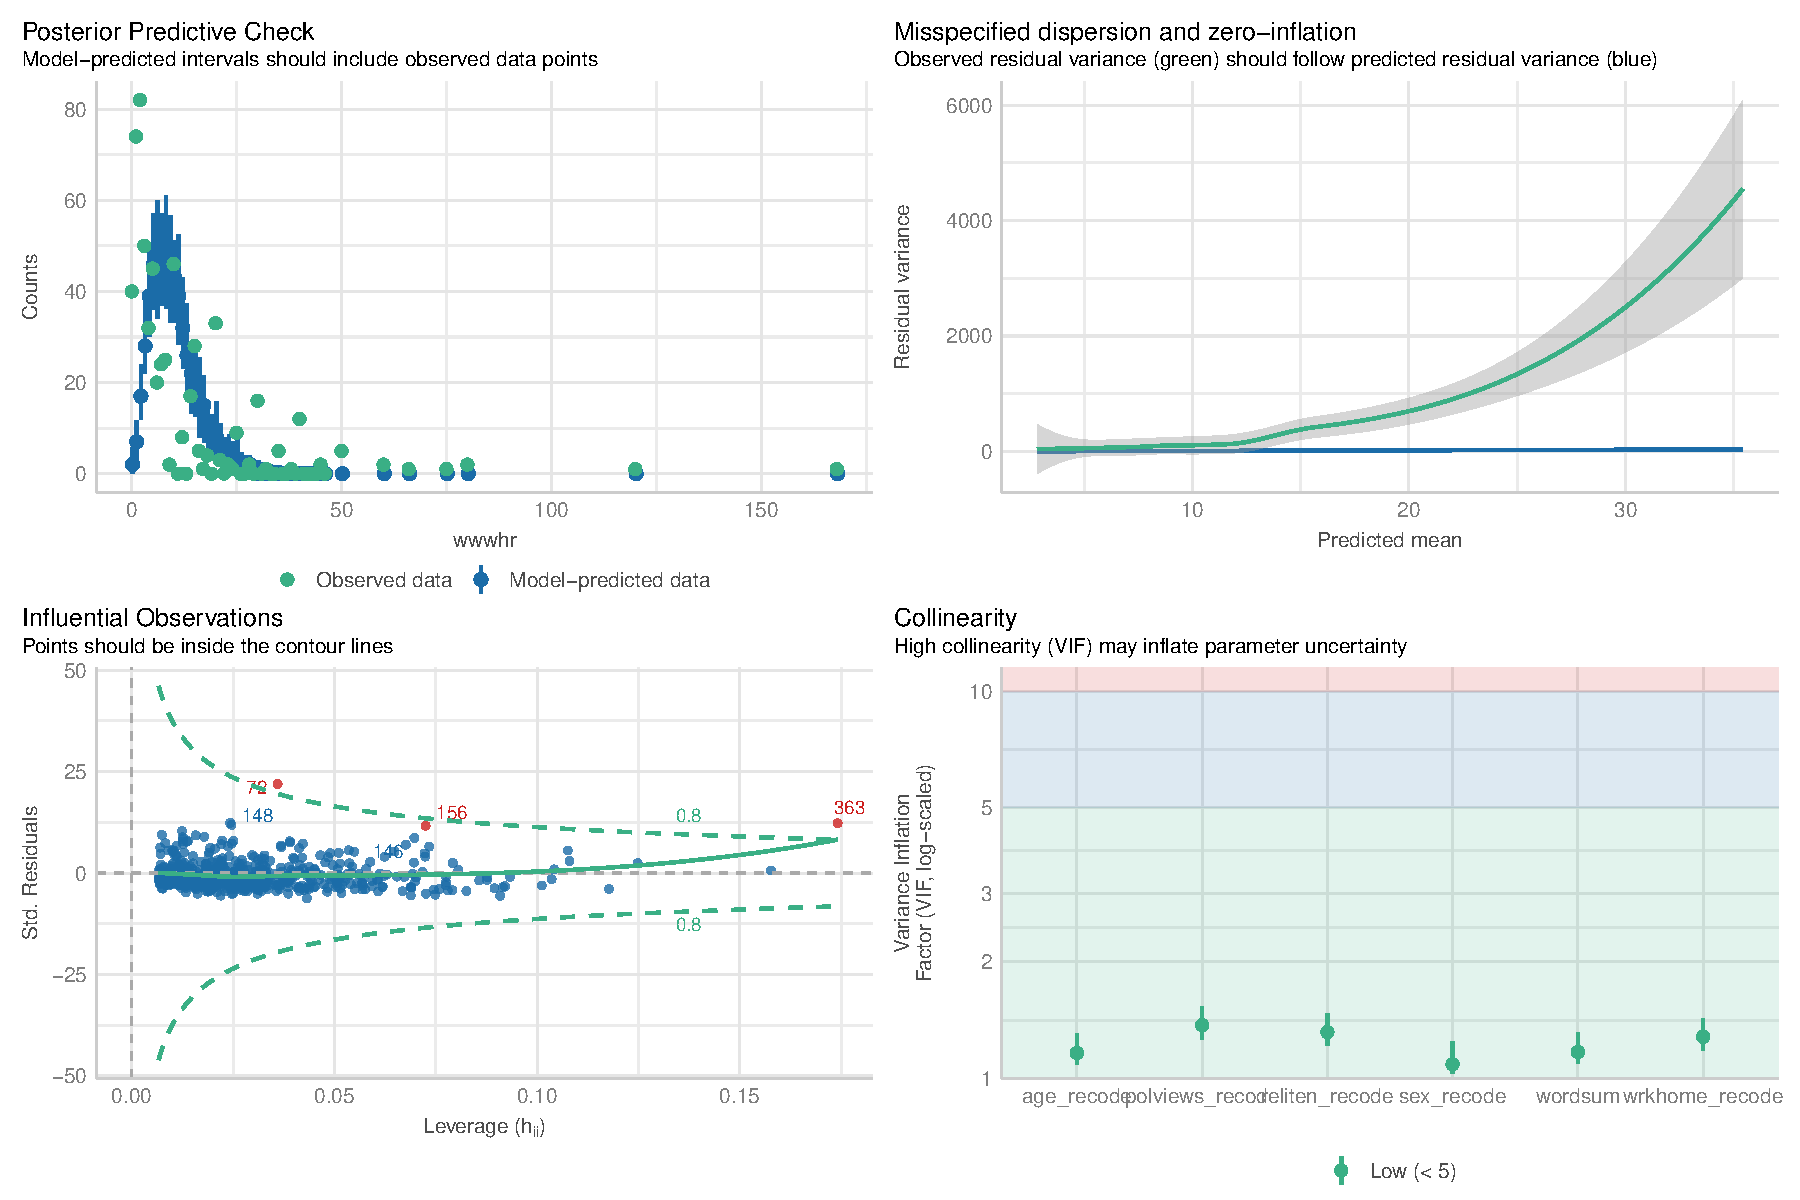
\includegraphics{poisson_lab_questions-1_files/figure-pdf/unnamed-chunk-7-1.pdf}

\subsection{Find any outliers}\label{find-any-outliers}

\begin{Shaded}
\begin{Highlighting}[]
\NormalTok{outlier\_idx }\OtherTok{=} \FunctionTok{check\_outliers}\NormalTok{(model1)}
\NormalTok{outlier\_idx}
\end{Highlighting}
\end{Shaded}

\begin{verbatim}
3 outliers detected: cases 72, 156, 363.
- Based on the following method and threshold: cook (0.8).
- For variable: (Whole model).
\end{verbatim}

\subsection{Refit the model after excluding
outliers}\label{refit-the-model-after-excluding-outliers}

\begin{Shaded}
\begin{Highlighting}[]
\NormalTok{data\_pos2 }\OtherTok{=}\NormalTok{ data\_pos }\SpecialCharTok{\%\textgreater{}\%}
  \FunctionTok{filter}\NormalTok{(}\SpecialCharTok{!} \FunctionTok{row\_number}\NormalTok{() }\SpecialCharTok{\%in\%} \FunctionTok{which}\NormalTok{(outlier\_idx))}

\NormalTok{model2 }\OtherTok{=} \FunctionTok{glm}\NormalTok{(wwwhr}\SpecialCharTok{\textasciitilde{}}\NormalTok{age}\SpecialCharTok{+}\NormalTok{wordsum}\SpecialCharTok{+}\NormalTok{sex\_recode}\SpecialCharTok{+}\NormalTok{reliten\_recode}\SpecialCharTok{+}\NormalTok{polviews\_recode}\SpecialCharTok{+}\NormalTok{wrkhome\_recode, }
              \AttributeTok{data=}\NormalTok{data\_pos2,}
              \AttributeTok{family=}\FunctionTok{poisson}\NormalTok{(}\AttributeTok{link=}\StringTok{"log"}\NormalTok{))}
\end{Highlighting}
\end{Shaded}

\begin{Shaded}
\begin{Highlighting}[]
\FunctionTok{model\_parameters}\NormalTok{(model2) }\SpecialCharTok{\%\textgreater{}\%}
  \FunctionTok{print\_html}\NormalTok{()}
\end{Highlighting}
\end{Shaded}

\begin{table}
\fontsize{12.0pt}{14.4pt}\selectfont
\begin{tabular*}{\linewidth}{@{\extracolsep{\fill}}lccccc}
\toprule
Parameter & Coefficient & SE & 95\% CI & z & p \\ 
\midrule\addlinespace[2.5pt]
{(Intercept)} & 1.89 & 0.09 & (1.71, 2.07) & 20.52 & < .001 \\ 
{age} & -0.02 & 1.10e-03 & (-0.02, -0.01) & -15.29 & < .001 \\ 
{wordsum} & 0.10 & 7.86e-03 & (0.08, 0.11) & 12.38 & < .001 \\ 
{sex recode (1)} & 0.22 & 0.03 & (0.17, 0.27) & 8.13 & < .001 \\ 
{reliten recode (2)} & 0.34 & 0.04 & (0.26, 0.41) & 8.88 & < .001 \\ 
{reliten recode (3)} & 0.43 & 0.06 & (0.30, 0.55) & 6.68 & < .001 \\ 
{reliten recode (4)} & 0.65 & 0.04 & (0.57, 0.72) & 16.23 & < .001 \\ 
{polviews recode (2)} & -0.10 & 0.07 & (-0.23, 0.03) & -1.49 & 0.136  \\ 
{polviews recode (3)} & -0.18 & 0.07 & (-0.31, -0.04) & -2.51 & 0.012  \\ 
{polviews recode (4)} & -0.21 & 0.06 & (-0.33, -0.08) & -3.23 & 0.001  \\ 
{polviews recode (5)} & -0.06 & 0.07 & (-0.19, 0.07) & -0.92 & 0.359  \\ 
{polviews recode (6)} & -0.25 & 0.07 & (-0.39, -0.11) & -3.46 & < .001 \\ 
{polviews recode (7)} & -0.31 & 0.10 & (-0.51, -0.11) & -3.02 & 0.003  \\ 
{wrkhome recode (2)} & 0.21 & 0.04 & (0.12, 0.29) & 4.57 & < .001 \\ 
{wrkhome recode (3)} & 0.35 & 0.05 & (0.26, 0.44) & 7.50 & < .001 \\ 
{wrkhome recode (4)} & 0.44 & 0.04 & (0.35, 0.52) & 9.76 & < .001 \\ 
{wrkhome recode (5)} & 0.24 & 0.04 & (0.15, 0.32) & 5.64 & < .001 \\ 
{wrkhome recode (6)} & 0.40 & 0.06 & (0.29, 0.51) & 7.20 & < .001 \\ 
\bottomrule
\end{tabular*}
\begin{minipage}{\linewidth}
\\
\end{minipage}
\end{table}

\subsubsection{Check for Overdispersion}\label{check-for-overdispersion}

Hint: performance package has the function you're looking for

\begin{Shaded}
\begin{Highlighting}[]
\NormalTok{performance}\SpecialCharTok{::}\FunctionTok{check\_overdispersion}\NormalTok{(model2)}
\end{Highlighting}
\end{Shaded}

\begin{verbatim}
# Overdispersion test

       dispersion ratio =   15.102
  Pearson's Chi-Squared = 8804.224
                p-value =  < 0.001
\end{verbatim}

What do you notice? And what's a good next step forward? Can there be
another model class that can fit the data? If so, fit this model to the
data.

\begin{itemize}
\tightlist
\item
  There is overdispersion, which means there is more variation in the
  response than what's implied by a Poisson model. We can try to fit a
  negative-binomial regression model.
\end{itemize}

\begin{Shaded}
\begin{Highlighting}[]
\NormalTok{model3 }\OtherTok{=} \FunctionTok{glm.nb}\NormalTok{(wwwhr}\SpecialCharTok{\textasciitilde{}}\NormalTok{age}\SpecialCharTok{+}\NormalTok{wordsum}\SpecialCharTok{+}\NormalTok{sex\_recode}\SpecialCharTok{+}\NormalTok{reliten\_recode}\SpecialCharTok{+}\NormalTok{polviews\_recode}\SpecialCharTok{+}\NormalTok{wrkhome\_recode, }
              \AttributeTok{data=}\NormalTok{data\_pos2)}

\NormalTok{model4 }\OtherTok{=}\NormalTok{ MASS}\SpecialCharTok{::}\FunctionTok{glm.nb}\NormalTok{(wwwhr}\SpecialCharTok{\textasciitilde{}}\NormalTok{age}\SpecialCharTok{+}\NormalTok{wordsum}\SpecialCharTok{+}\NormalTok{sex\_recode}\SpecialCharTok{+}\NormalTok{reliten\_recode}\SpecialCharTok{+}\NormalTok{polviews\_recode}\SpecialCharTok{+}\NormalTok{wrkhome\_recode, }
              \AttributeTok{data=}\NormalTok{data\_pos2)}
\end{Highlighting}
\end{Shaded}

\subsection{Which one is better- your earlier model, or later
model?}\label{which-one-is-better--your-earlier-model-or-later-model}

\begin{Shaded}
\begin{Highlighting}[]
\FunctionTok{test\_likelihoodratio}\NormalTok{(model2, model3) }\SpecialCharTok{\%\textgreater{}\%}
  \FunctionTok{kable}\NormalTok{()}
\end{Highlighting}
\end{Shaded}

\begin{longtable}[]{@{}lllrrrr@{}}
\toprule\noalign{}
& Name & Model & df & df\_diff & Chi2 & p \\
\midrule\noalign{}
\endhead
\bottomrule\noalign{}
\endlastfoot
model2 & model2 & glm & 18 & NA & NA & NA \\
model3 & model3 & negbin & 19 & 1 & 4510.038 & 0 \\
\end{longtable}

\begin{Shaded}
\begin{Highlighting}[]
\FunctionTok{test\_likelihoodratio}\NormalTok{(model2, model4) }\SpecialCharTok{\%\textgreater{}\%}
  \FunctionTok{kable}\NormalTok{()}
\end{Highlighting}
\end{Shaded}

\begin{longtable}[]{@{}lllrrrr@{}}
\toprule\noalign{}
& Name & Model & df & df\_diff & Chi2 & p \\
\midrule\noalign{}
\endhead
\bottomrule\noalign{}
\endlastfoot
model2 & model2 & glm & 18 & NA & NA & NA \\
model4 & model4 & negbin & 19 & 1 & 4510.038 & 0 \\
\end{longtable}

The later model is better here, which means the previous poisson model
was not a good fit to the data.

\subsection{What is zero inflation? Is there zero-inflation in your
chosen
model?}\label{what-is-zero-inflation-is-there-zero-inflation-in-your-chosen-model}

\begin{Shaded}
\begin{Highlighting}[]
\NormalTok{performance}\SpecialCharTok{::}\FunctionTok{check\_zeroinflation}\NormalTok{(model3)}
\end{Highlighting}
\end{Shaded}

\begin{verbatim}
# Check for zero-inflation

   Observed zeros: 40
  Predicted zeros: 67
            Ratio: 1.68
\end{verbatim}

There is no zero-inflation here since \# of observed zeros \textless{}
\# of predicted zeros.

\subsection{Log Lambda}

\begin{Shaded}
\begin{Highlighting}[]
\FunctionTok{print}\NormalTok{(}\FunctionTok{coef}\NormalTok{(model4))}
\end{Highlighting}
\end{Shaded}

\begin{verbatim}
     (Intercept)              age          wordsum      sex_recode1 
      1.72933133      -0.01630350       0.10573220       0.14429163 
 reliten_recode2  reliten_recode3  reliten_recode4 polviews_recode2 
      0.28114285       0.38546776       0.62578244       0.17573144 
polviews_recode3 polviews_recode4 polviews_recode5 polviews_recode6 
      0.09431515      -0.04193018       0.13914802      -0.04427420 
polviews_recode7  wrkhome_recode2  wrkhome_recode3  wrkhome_recode4 
     -0.15510946       0.11140958       0.31377893       0.30530537 
 wrkhome_recode5  wrkhome_recode6 
      0.15257360       0.25947760 
\end{verbatim}

\begin{Shaded}
\begin{Highlighting}[]
\FunctionTok{print}\NormalTok{(}\FunctionTok{exp}\NormalTok{(}\FunctionTok{coef}\NormalTok{(model4)))}
\end{Highlighting}
\end{Shaded}

\begin{verbatim}
     (Intercept)              age          wordsum      sex_recode1 
       5.6368834        0.9838287        1.1115242        1.1552210 
 reliten_recode2  reliten_recode3  reliten_recode4 polviews_recode2 
       1.3246428        1.4703019        1.8697083        1.1921179 
polviews_recode3 polviews_recode4 polviews_recode5 polviews_recode6 
       1.0989060        0.9589367        1.1492942        0.9566916 
polviews_recode7  wrkhome_recode2  wrkhome_recode3  wrkhome_recode4 
       0.8563214        1.1178527        1.3685871        1.3570393 
 wrkhome_recode5  wrkhome_recode6 
       1.1648282        1.2962527 
\end{verbatim}

\begin{Shaded}
\begin{Highlighting}[]
\FunctionTok{mean}\NormalTok{(}\FunctionTok{exp}\NormalTok{(}\FunctionTok{predict}\NormalTok{(model4, }\AttributeTok{type =} \StringTok{"link"}\NormalTok{)))}
\end{Highlighting}
\end{Shaded}

\begin{verbatim}
[1] 9.879506
\end{verbatim}

\subsection{Mean Count}

\begin{Shaded}
\begin{Highlighting}[]
\FunctionTok{print}\NormalTok{(}\FunctionTok{mean}\NormalTok{(data\_pos2}\SpecialCharTok{$}\NormalTok{wwwhr, }\AttributeTok{na.rm =} \ConstantTok{TRUE}\NormalTok{))}
\end{Highlighting}
\end{Shaded}

\begin{verbatim}
[1] 9.792543
\end{verbatim}

\begin{Shaded}
\begin{Highlighting}[]
\NormalTok{data\_pos\_base }\OtherTok{=}\NormalTok{ data\_pos2 }\SpecialCharTok{\%\textgreater{}\%}
  \FunctionTok{filter}\NormalTok{(sex\_recode}\SpecialCharTok{=={-}}\DecValTok{1}\NormalTok{, reliten\_recode}\SpecialCharTok{==}\DecValTok{1}\NormalTok{, polviews\_recode}\SpecialCharTok{==}\DecValTok{1}\NormalTok{, wrkhome\_recode}\SpecialCharTok{==}\DecValTok{1}\NormalTok{)}
\FunctionTok{mean}\NormalTok{(data\_pos\_base}\SpecialCharTok{$}\NormalTok{wwwhr, }\AttributeTok{na.rm =} \ConstantTok{TRUE}\NormalTok{)}
\end{Highlighting}
\end{Shaded}

\begin{verbatim}
[1] 5.4
\end{verbatim}

\subsection{Report your conclusions}\label{report-your-conclusions}

The coefficients of the model is roughly similar to the log value of the
mean of the dependent variable. The exponential of the intercept of the
model is 5.637, while the mean number of hours per week that a person
spends on the internet (wwwhr) for the baseline group (sex=-1,
religosity=1, political\_orientation=1, work\_from\_home=1) is 5.4.

Because of the numerous number of levels for different categorical
variables, here we don't look at each different levels. We can use our
full model to predict the dependent variable, and then take the mean of
the exponential, which is 9.880, while the mean wwwhr for the whole
dataset is 9.793.

Overall, a negative-binomial regression model is a good fit to the data
due to dispersion. We don't need to use a zero-inflated model since
there is no zero-inflation.



\end{document}
